\documentclass{beamer}
\usepackage[latin1, utf8]{inputenc}
\usepackage{wrapfig}
\usepackage{framed}

\useoutertheme[height=0pt,left]{sidebar}
\usecolortheme{seahorse}
\setbeamercolor*{titlelike}{parent=structure}
\useinnertheme{circles}
\setbeamertemplate{frametitle}[default][right]

\title{Les robots ressemblant à l'humain sont-ils vraiment utiles ?}
\author{Christian LASSERRE\\ Théophile GUILBAUD}
\institute{ENSEIRB-MATMECA}
\date{}

\begin{document}
\begin{frame}
  \titlepage
\end{frame}

\begin{frame}
  \tableofcontents
\end{frame}

\section{Ressemblance}
\begin{frame}
  RESSEMBLANCE
\end{frame}

\subsection{Le(s) Géminoide(s)}
\begin{frame}{Histoire}
  Professeur
\end{frame}

\begin{frame}{Auteur}
\end{frame}

\subsection{Caractéristiques}
\begin{frame}{Geminoide HI-4}
  \begin{framed}
    \begin{wrapfigure}{l}{40mm}
      \centering
      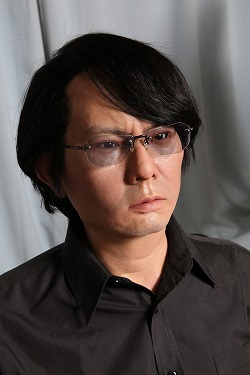
\includegraphics[width=40mm]{data/HI-4}
      \caption{Geminoïde HI-4}
    \end{wrapfigure}
    Il était une fois ...
  \end{framed}
\end{frame}

\begin{frame}{Geminoide HI-2}
\end{frame}

\begin{frame}{Geminoide F}
  (il y a aussi le DK...)
  convention social -> uniquement physique
\end{frame}

\subsection{Conclusion}
\begin{frame}{ça ressemble à un humain}
\end{frame}

\section{L'intéraction}
\begin{frame}
  INTERACTION
\end{frame}

\subsection{Télénoïde}
\begin{frame}{Présentation}
  \begin{framed}
	\begin{wrapfigure}{l}{40mm}
		\centering
		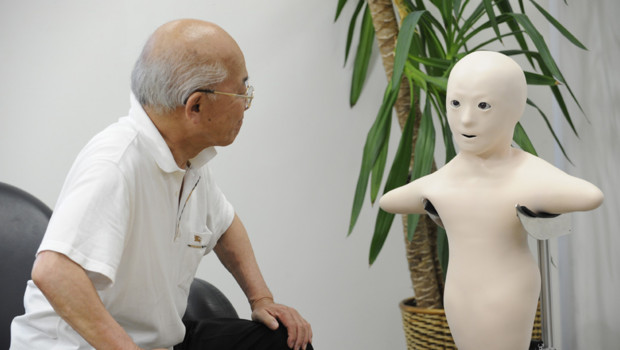
\includegraphics[width=0.05]{data/telenoid}
		\caption{Le robot Telenoide}
    \end{wrapfigure}
  \end{framed}  
  Le robot qui transfère votre présence
\end{frame}

\begin{frame}{Caractéristiques}
  \begin{itemize}
  \item 7 versions (depuis aout 2010)
  \item taille : 50cm
  \item poids : 3.5kg
  \item capteurs : 2 microphones
  \item alimentation : batterie
  \item degré de liberté
	\begin{itemize}
	\item 3 sur les yeux
	\item 1 sur la bouche
	\item 3 sur le coup
	\item 2 sur les moignons
	\end{itemize}
  \item peau en PVC
  \item prix 35.000\$ les premiers (environ 8.000\$ desormais)
  \end{itemize}
\end{frame}

\subsection{Utilité}
\begin{frame}
Design androgyne pour permettre la diversité des utilisateurs
\vspace{0.5cm}
Pas encore assez de capteurs
\vspace{0.5cm}
C'est un téléphone qui a pour but de transmettre a présence

  \begin{itemize}
  \item possibilité d'utilisation futur :
	  \begin{itemize}
	  \item accueil hotel/aéroport
	  \item sex-symbol
	  \item ...
	  \end{itemize}
  \end{itemize}
\end{frame}

\begin{frame}{Avenir}
  Le robot qui nous permettra l'ubiquité
\vspace{0.5cm}  
VIDEO
\end{frame}

\subsection{Conclusion}
\begin{frame}
  Robot Inhabituel, contre exemple de ce qu'on attend d'un robot.
  Aucune étude de proxémie, convention sociale développée, etc...
\end{frame}

\end{document}
